
%%%%%%%%%%%%%%%%%%%%%%%%%%%%%%%%%%%%%%%%%%%%%%%%%%%%%%%%%%%%%%%%%%%%%%%%%%%%%%%%%%%%%%%
%%%%%%%%%%%%%%%%%%%%%%%%%%%%%%%%%%%%%%%%%%%%%%%%%%%%%%%%%%%%%%%%%%%%%%%%%%%%%%%%%%%%%%%
% 
% This top part of the document is called the 'preamble'.  Modify it with caution!
%
% The real document starts below where it says 'The main document starts here'.

\documentclass[12pt]{article}

\usepackage{amssymb,amsmath,amsthm}
\usepackage[top=1in, bottom=1in, left=1.25in, right=1.25in]{geometry}
\usepackage{fancyhdr}
\usepackage{enumerate}
\usepackage{listings}
\usepackage{graphicx}
\usepackage{float}
\usepackage{multicol}
% Comment the following line to use TeX's default font of Computer Modern.
\usepackage{times,txfonts}
\usepackage{mwe}
\usepackage{caption}
\usepackage{subcaption}
\usepackage{svg}





\makeatletter
\renewcommand*\env@matrix[1][*\c@MaxMatrixCols c]{%
  \hskip -\arraycolsep
  \let\@ifnextchar\new@ifnextchar
  \array{#1}}
\makeatother

\newtheoremstyle{homework}% name of the style to be used
  {18pt}% measure of space to leave above the theorem. E.g.: 3pt
  {12pt}% measure of space to leave below the theorem. E.g.: 3pt
  {}% name of font to use in the body of the theorem
  {}% measure of space to indent
  {\bfseries}% name of head font
  {:}% punctuation between head and body
  {2ex}% space after theorem head; " " = normal interword space
  {}% Manually specify head
\theoremstyle{homework} 

% Set up an Exercise environment and a Solution label.
\newtheorem*{exercisecore}{Exercise \@currentlabel}
\newenvironment{exercise}[1]
{\def\@currentlabel{#1}\exercisecore}
{\endexercisecore}

\newcommand{\localhead}[1]{\par\smallskip\noindent\textbf{#1}\nobreak\\}%
\newcommand\solution{\localhead{Solution:}}

%%%%%%%%%%%%%%%%%%%%%%%%%%%%%%%%%%%%%%%%%%%%%%%%%%%%%%%%%%%%%%%%%%%%%%%%
%
% Stuff for getting the name/document date/title across the header
\makeatletter
\RequirePackage{fancyhdr}
\pagestyle{fancy}
\fancyfoot[C]{\ifnum \value{page} > 1\relax\thepage\fi}
\fancyhead[L]{\ifx\@doclabel\@empty\else\@doclabel\fi}
\fancyhead[C]{\ifx\@docdate\@empty\else\@docdate\fi}
\fancyhead[R]{\ifx\@docauthor\@empty\else\@docauthor\fi}
\headheight 15pt

\def\doclabel#1{\gdef\@doclabel{#1}}
\doclabel{Use {\tt\textbackslash doclabel\{MY LABEL\}}.}
\def\docdate#1{\gdef\@docdate{#1}}
\docdate{Use {\tt\textbackslash docdate\{MY DATE\}}.}
\def\docauthor#1{\gdef\@docauthor{#1}}
\docauthor{Use {\tt\textbackslash docauthor\{MY NAME\}}.}
\makeatother



\usepackage{mathabx}





% Shortcuts for blackboard bold number sets (reals, integers, etc.)
\newcommand{\Reals}{\ensuremath{\mathbb R}}
\newcommand{\Nats}{\ensuremath{\mathbb N}}
\newcommand{\Ints}{\ensuremath{\mathbb Z}}
\newcommand{\Rats}{\ensuremath{\mathbb Q}}
\newcommand{\Cplx}{\ensuremath{\mathbb C}}
%% Some equivalents that some people may prefer.
\let\RR\Reals
\let\NN\Nats
\let\II\Ints
\let\CC\Cplx

%%%%%%%%%%%%%%%%%%%%%%%%%%%%%%%%%%%%%%%%%%%%%%%%%%%%%%%%%%%%%%%%%%%%%%%%%%%%%%%%%%%%%%%
%%%%%%%%%%%%%%%%%%%%%%%%%%%%%%%%%%%%%%%%%%%%%%%%%%%%%%%%%%%%%%%%%%%%%%%%%%%%%%%%%%%%%%%
% 
% The main document start here.

% The following commands set up the material that appears in the header.
\doclabel{Math 614: Homework 7}
\docauthor{Stefano Fochesatto}
\docdate{\today}

\begin{document}


\begin{exercise}{P18} Suppose $A$ is a 100 by 100 matrix with $||A||_2 = 10$ and $||A||_F = 11$. Give the sharpest possible lower bound on 
  the 2-norm condition number of $A$.\\ 
  \solution First recall the definition for the 2-norm condition number of $A$ by theorem 12.15, 
  \begin{equation*}
    \kappa_2(A) =||A||_2*||A^{-1}||_2 = \dfrac{\sigma_1}{\sigma_{100}}. 
  \end{equation*}
  This definition recalls that $||A||_2 = \sigma_1 = 10$, similarly consider that $||A||_F$ is defined by, 
  \begin{equation*}
    ||A||_F =\sqrt{\sigma_1^2 + \dots + \sigma_{100}^2}
  \end{equation*} 
  Substituting the given value for $\sigma_1 = 10$ and $||A||_F = 11$ we get the following, 
  \begin{align*}
    11 &= \sqrt{10^2 + \dots + \sigma_{100}^2},\\
    121 &= 100 + \dots + \sigma_{100}^2,\\
    21 &= \sigma_2^2 + \dots + \sigma_{100}^2.
    \end{align*}
    Note that by definition, $\sigma_i$ is a monotone decreasing sequence therefore we get the following inequality, 
    \begin{align*}
      21 &= \sigma_2^2 + \dots + \sigma_{100}^2,\\
         &\geq \sigma_{100}^2 + \dots + \sigma_{100}^2,\\
         &\geq 99*\sigma_{100}^2,\\
       \dfrac{21}{99}  &\geq \sigma_{100}^2,\\
       \sqrt{\dfrac{21}{99}}&\geq \sigma_{100},\\
       \dfrac{1}{\sigma_{100}} &\geq \sqrt{\dfrac{99}{21}}.
    \end{align*}
    Finally substituting the final inequality into our definition of the 2-norm condition number we get a lower bound, 
    \begin{equation*}
      \kappa_2(A) = \dfrac{\sigma_1}{\sigma_{100}} \geq 10*\sqrt{\dfrac{99}{21}}.
    \end{equation*}  
\end{exercise}
\vspace{1in}



\begin{exercise}{P19} Consider the polynomial $p(x) = (x - 3)^{10} = x^{10}-30x^9+405x^8-3240x^7+17010x^6-61236x^5+153090x^4-262440x^3+295245x^2-196830x+59049.$\\
  \begin{enumerate}
    \item[a.] Plot $p(x)$ for $x = 2.85:.01:3.15$ evaluating $p(x)$ via it's coefficints.\\
    \solution Importing the coefficients of the expanded polynomial into matlab, we can evaluate it on the given x values using the polyval() function. Doing so we 
    get the following plot and code.
    \begin{figure}[H]
      \begin{center}
        \caption{Plot of $p(x)$ Evaluated by Coefficients}
         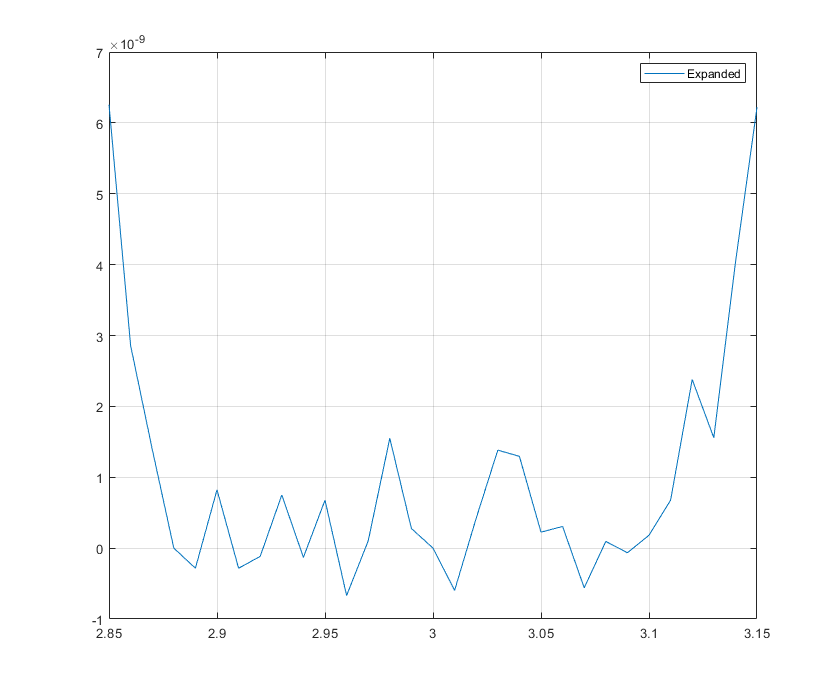
\includegraphics[width=.90\textwidth]{Fig01.png}
      \end{center}
    \end{figure}
    \textbf{Code:}
    \begin{center}
      \lstinputlisting{r1.txt}
    \end{center}


    \item[b.] Plot $p(x)$ again, now using its expression $(x - 3)^{10}$\\
    \solution Similarly we can do the same for the factored version of $p(x)$ and we get, 
    \begin{figure}[H]
      \begin{center}
        \caption{Plot of $p(x)$ Evaluated by $(x - 3)^{10}$}
         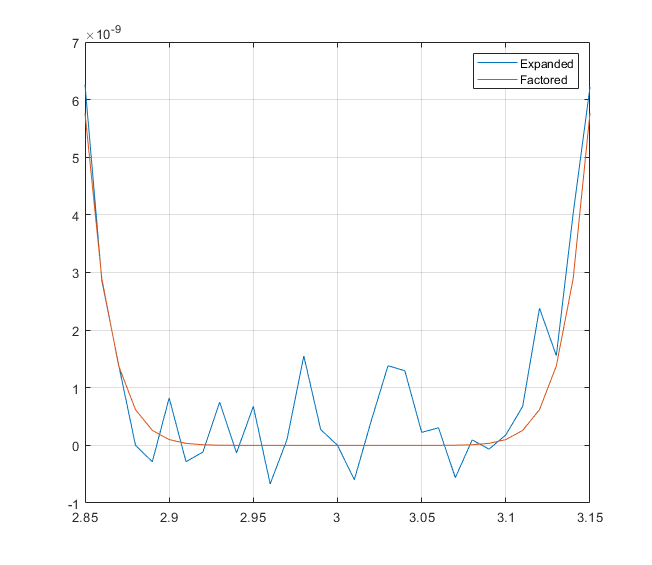
\includegraphics[width=.90\textwidth]{Fig1.png}
      \end{center}
    \end{figure}
    \textbf{Code:}
    \begin{center}
      \lstinputlisting{r2.txt}
    \end{center}

    











    \item[c.] In two or three sentences, compare and contrast the bad behavior here with the ill-conditioning phenomenon in 
    Example 12.5 on page 92. \\   
    \solution Example 12.5 describes the relationship and sensitivity between the coefficients of a polynomial, and the evaluation of it's roots. Note 
    that this could be applied to the evaluation of the polynomial across it's whole domain through elementary transformations, which seems to be the difference 
    in the two examples. Example 12.5 discusses applying a perturbation to the coefficient of a polynomial, in the previous problem we accomplished a similar situation 
    from the accumulation of rounding error (perturbing an ill-conditioned problem). Figure 12.1 shows the sensitivity of evaluating a polynomial via coefficints with 
    perturbations sampled from a normal distribution(and rounding error), the previous problem shows sensitivity to perturbation caused by rounding error. 
  \end{enumerate}
\end{exercise}
\vspace{1in}













\begin{exercise}{P20} Read the following 12 page encyclopedia entry: \\
L.N. Trefethen, Numerical Analysis , in W. T. Gowers, editor, Princeton\\
Companion to Mathematics, Princeton U. Press, 2008.\\
Answer the following questions with a sentence or wto at most: 
\begin{enumerate}
  \item[i.] Give a one-sentence version of Trefethen's definition of "numerical analysis"\\
  \solution It is the study of iterative and algorithimic methods for solving, or in reality approximating solutions to continuous problems in mathematics. 
  \item[ii.] Is analysis of rounding error the main business of numerical analysis? If not, what is?\\
  \solution Analysis of rounding error is an imporant aspect of numerical analysis, however a large marjority of numerical analysis 
  is related to designing and studying algorithms. Searching for stable algorithms which converge quickly and are performant. 
  \item[iii.] Gaussion elimatino with pivotoing as a matrix factorizaiont. State it. \\
  Gaussion elimination is also known a LU factoriztion, Gaussian elimination with pivoting involoves 
  a permutation matrix $P$ to reduce rounding error, 
  \begin{equation*}
    PA = LU.
  \end{equation*} 
  \item[iv.] Trefethen refers to Householdere Tiragularizaiton, Algorith, 10.1 in our text book, as 
  'QR factorization'. But then what does the 'QR algorithm' do?\\ 
  \solution The 'QR algorithm' that is discussed in the reading an iterative method for solving the eigenvalues of a matrix. We discussed 
  it in one aof the previous homeworks. 
  \item[v.]Which of the major 'algorithmic developmeents in history of numerical anlayis' have we already covered in MATH 614? \
  What do you think we will cover?\\
  \solution As we stated in the previous section he have briefly discussed some iterative methods like the 'QR algorithm'. We have also discussed the different 
  matrix ortoginalizations, Householder, and GramShmidt. I think that looking forward we will delve further into the iterative methods for eigen values and solutions to 
  linear equations. 
  \item[vi.] What is the 'central dogma' of numerical linear algebra?\\
  \solution The central dogma, or guiding principles of numerical linear algebra are matrix factorizations and algorithms.  
\end{enumerate}
\end{exercise}









\begin{exercise}[12.2] In Example 11.1 we remarked that polynomial interpoloation in equi-spaced points 
  is ill-conditioned. To illustrate this phenomoenon, let $x_1, \dots x_n$ and  $y_1, \dots y_m$ be n and m equispaced points form 
  -1 to 1 respectively.\\
  \begin{enumerate}
    \item[a.] Derive a formula for the $mxn$ matrix $A$ that maps an $n$-vector of data at $\{x_j\}$ to an 
    m vector of sampled values $\{p(y_j)\}$, where $p$ is the degree $n-1$ polynomial interpolant of the data.\\
   
    \solution First let $\hat{x}$ be an n-vector of data at $x$ values and note that A must have the following property,
    \begin{equation*}
      A\hat{x} = p(y). 
    \end{equation*} 
    Where $p(y)$ is an m-vector of sampled values from the $n-1$ polynomial interpolant of $\hat{x}$. Now consider the $n-1$ polynomial interpolation (by 11.1) 
    which transforms $x$ to $\hat{x}$
    \begin{equation*}
      X\hat{c} = 
      \begin{bmatrix}
        1 & x_1 & x_1^2 & \cdots & x_1^{n-1} \\
        \vdots & \vdots & \vdots & \ddots &\vdots \\
        1 & x_n & x_n^2 & \cdots & x_n^{n-1} \\ 
        \end{bmatrix}
        \begin{bmatrix}
          c_1\\
          \vdots \\
          c_{n-1}
          \end{bmatrix}
           = \hat{x}
    \end{equation*}
    Note that $\hat{c}$ are the coefficient to the polynomial interpolant. Now consider the same transformation but instead applied to an m-vector $y$, to produce $p(y)$,
        \begin{equation*}
      Y\hat{c} = 
      \begin{bmatrix}
        1 & y_1 & y_1^2 & \cdots & y_1^{n-1} \\
        \vdots & \vdots & \vdots & \ddots &\vdots \\
        1 & y_m & y_m^2 & \cdots & y_m^{n-1} \\ 
        \end{bmatrix}
        \begin{bmatrix}
          c_1\\
          \vdots \\
          c_{n-1}
          \end{bmatrix}
           = p(y).
    \end{equation*}
    Substituting into our original equation, we can solve for $A$, 
    \begin{align*}
      A\hat{x} &= p(y)\\
      AX\hat{c} &= Y\hat{c}
    \end{align*}
    From here we can see that the equality holds when $A = YX^{-1}$.
    \vspace{.25in}



    \item[b.] Write a prgram to calcuate $A$ and plot $||A||_{\infty}$ on a semilog scale for $n = 1:30$ and $m = 2n-1$. 
    In teh continous limie as m goes to infinity, the numbers of $||A||_{\infty}$ are know as teh Lebesque constatns for equispaced 
    interpolation, which are asymptotoic to $2^n/(e(n-1)logn)$ and $n$ goes to infinty. \\
    \solution Consider the following Matlab code, \\
    \begin{figure}[H]
      \begin{center}
        \caption{$||A||_{\infty}$ plotted over $n = 1:30$}
         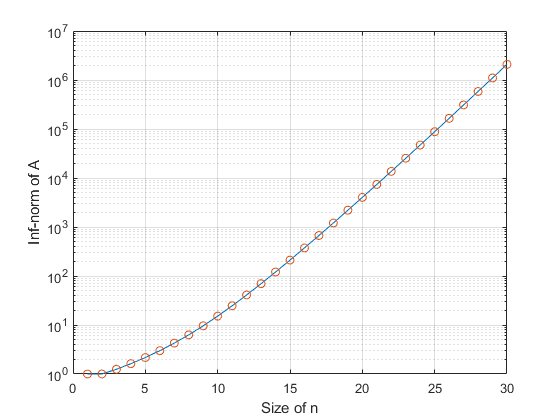
\includegraphics[width=.90\textwidth]{Fig3.png}
      \end{center}
    \end{figure}
    \textbf{Code:}
    \begin{center}
      \lstinputlisting{r3.txt}
    \end{center}
    \vspace{.25in}


    \item[c.] For $n = 1:30$, and $m = 2n - 1$ what is the infinity norm condition number $k$ of the proble,m of interpolating 
    the constant function 1? Use (12.6)\\
    \solution Recall the definition of the infinity norm condition number from 12.6, 
    \begin{equation*}
      \kappa = \dfrac{||J||_{\infty}}{||f(x)||_{\infty}/ ||x||_{\infty}}
    \end{equation*}
    Where $f(x) = Ax$. Note that $A$ is meant to map data $\hat{x}$ from a corresponding $x$ to sampled values $p(y)$ from a corresponding y where $\hat{x}$ and $p(y)$
    must lie on the constant function 1. Therefore since 
    A is mapping a constant function we know that,
    \begin{equation*}
      ||x||_{\infty} = \max{|\hat{x}_n|} = 1
    \end{equation*}
    \begin{equation*}
      ||f(x)||_{\infty} = \max{|p(y)_m|} = 1
    \end{equation*}
    Note that since $A$ is a constant matrix $J(x) = A$, and by substitution we get, 
    \begin{equation*}
      \kappa = \dfrac{||J||_{\infty}}{||f(x)||_{\infty}/ ||x||_{\infty}} = \dfrac{||A||_{\infty}}{1/1} = ||A||_{\infty}.
    \end{equation*}
    \vspace{.25in}




    item[d.] How close is your result for $n = 11$ to the bound implicit in Figure 11.1?\\
    \solution We can see our result for the infinity norm condition number of $A$ $n = 11$ from the code in part B. We can see that the 
    figure in 11.1 has a bound of approximately 4, and our result for the infinity norm condition number came out to approximately 24.661,
    \textbf{Console:}
    \begin{center}
      \lstinputlisting{r4.txt}
    \end{center}
    \vspace{.25in}
    


  \end{enumerate}
\end{exercise}
  \vspace{1in}




  \begin{exercise}{13.2} The floating point system $F$ defined by 13.2 includes many integers, but not all of them\\
    \begin{enumerate}
      \item[a.] Give an exact formula for the smallest positive integer that does not belong to $F$. \\
      \solution From the formula given in (13.2) every value in $F$ has the form, 
      \begin{equation*}
        x = \pm \frac{m}{\beta^t}\beta^e = \pm m\beta^{e-t}
      \end{equation*}
      Note that $m$ is an integer in the rangfe of $1 \leq m \leq \beta^t$. If we let $e = t$ we get that $x = \pm m \leq \beta^2 $. So 
      $n = \beta^t + 1$ becomes the smallest integer just outside that range. 

      \item[b.] In particular, what are the values of $n$ for IEEE single  and double precision arithmetic?\\
      \solution For single presizino arithmetic we know that the $precision$, or $t = 24$ so, 
      \begin{equation*}
        n = 2^{24} + 1 = 16777217
      \end{equation*}
      For double precision arithmetic we ge that the $precision$ is $t = 53$ so, 
      \begin{equation*}
        n = 2^{53} + 1 = 9007199254740993
      \end{equation*}
    \end{enumerate}  
  \end{exercise}
  \vspace{1in}


  \begin{exercise}{14.1} True or False?\\
    \begin{enumerate}
      \item[a.] $\sin(x) = O(1)$ as $x \to \infty$\\
      \solution True. $\sin(x)$ is a periodic and bounded function whose output is always $|\sin(x)| \leq 1$.
      \item[b.] $\sin(x) = O(1)$ as $x \to 0$\\
      \solution True. As $x \to 0$ we know that $|\sin(x)| \leq 1$. 
      \item[c.] $log(x) = O(x^{1/100})$ as $x \to \infty$\\
      \solution  True, Consider that $log(x)<x$ as $x \to \infty$. Note that all function are increasing as $x \to \infty$, so composition yields, 
      \begin{equation*}
      log(x^{1/100}) < x^{1/100},
    \end{equation*}
    \begin{equation*}
      log(x) < 100x^{1/100}.
    \end{equation*}
      \item[e.] $A = O(V^{2/3})$ as $V \to \infty$, where $A$ and $V$ are the surface area and volume of a 
      sphere measured in square miles and cubic microns, respectively. \\
      \solution True, recall that the surface area of a sphere is measured by, 
      \begin{equation*}
        A = 4\pi r^2 = O(r^2)
      \end{equation*}
      and that the volume of a sphere is measured by, 
      \begin{equation*}
        V = \frac{4}{3}\pi r^3
      \end{equation*}
      Note that there is some dimensional analysis constant which facilitates comparison between square miles and cubic micros, which is oppressed by 
      big O notation. Consider $V^{2/3}$
      \begin{equation*}
        V^{2/3} = (\frac{4}{3}\pi)^{2/3} r^2 = O(r^2) = A.
      \end{equation*}
      \item[f.] $fl(\pi) - \pi = O(\epsilon_{machine})$\\
      \solution True. By definition 13.5, $fl(\pi) - \pi \leq \epsilon_{machine}$ .
    \end{enumerate}
    
  \end{exercise}













\end{document}




















